\section{Evaluation}
\begin{itemize}
  \item How they all come together
  \item Examples of TPM commands with session types
\end{itemize}

\subsection{TPM as Session Types}

$\left\{
\begin{tabular}{ l }
	\textit{Read}: \enspace Alice $\rightarrow$ TPM : Read. PCR $\rightarrow$ TPM : vlaue. TPM $\rightarrow$ PCR : value. TPM $\rightarrow$ Alice : value \\
	\textit{Quote}: \enspace Alice $\rightarrow$ TPM : Quote. PCR $\rightarrow$ TPM : value. TPM $\rightarrow$ PCR : value TPM $\rightarrow$ Alice : CertPCR\\
	\textit{CreateWrapKey}: \enspace Alice $\rightarrow$ TPM : CreateWrapKey. PCR $\rightarrow$ TPm : value. TPM $\rightarrow$ PCR : value. KeyTable $\rightarrow$ TPM : KeyLoaded. ?(new key)?. TPM $\rightarrow$ Alice : data\\
	\textit{LoadKey2}: \enspace Alice $\rightarrow$ TPM : LoadKey2. PCR $\rightarrow$ TPM : value. TPM $\rightarrow$ PCR : value. KeyTable $\rightarrow$ TPM : KeyLoaded. TPM $\rightarrow$ KeyTable : KeyLoaded\\
	\textit{CertifyKey}: \enspace Alice $\rightarrow$ TPM : data. KeyTable $\rightarrow$ TPM : KeyLoaded. TPM $\rightarrow$ Alice : Cert \\
	\textit{Unbind}: \enspace Alice $\rightarrow$ TPM : unbind. PCR $\rightarrow$ TPM : value. TPM $\rightarrow$ PCR : value. KeyTable $\rightarrow$ TPM : KeyLoaded. TPM $\rightarrow$ Alice : adec\\
	\textit{Seal}: \enspace Alice $\rightarrow$ TPM : data. PCR $\rightarrow$ TPM : value. TPM $\rightarrow$ PCR : value. KeyTable $\rightarrow$ TPM : KeyLoaded. TPM $\rightarrow$ Alice : data\\
	\textit{Unseal}: \enspace Alice $\rightarrow$ TPM : unseal. PCR $\rightarrow$ TPM : value. TPM $\rightarrow$ PCR : value. KeyTable $\rightarrow$ TPM : KeyLoaded. TPM $\rightarrow$ Alice : KeyLoaded\\
	\textit{Extend}: \enspace Alice $\rightarrow$ TPM : extend. PCR $\rightarrow$ TPM : value. TPm $\rightarrow$ PCR : hpcr
\end{tabular}
\right.$

\begin{center}
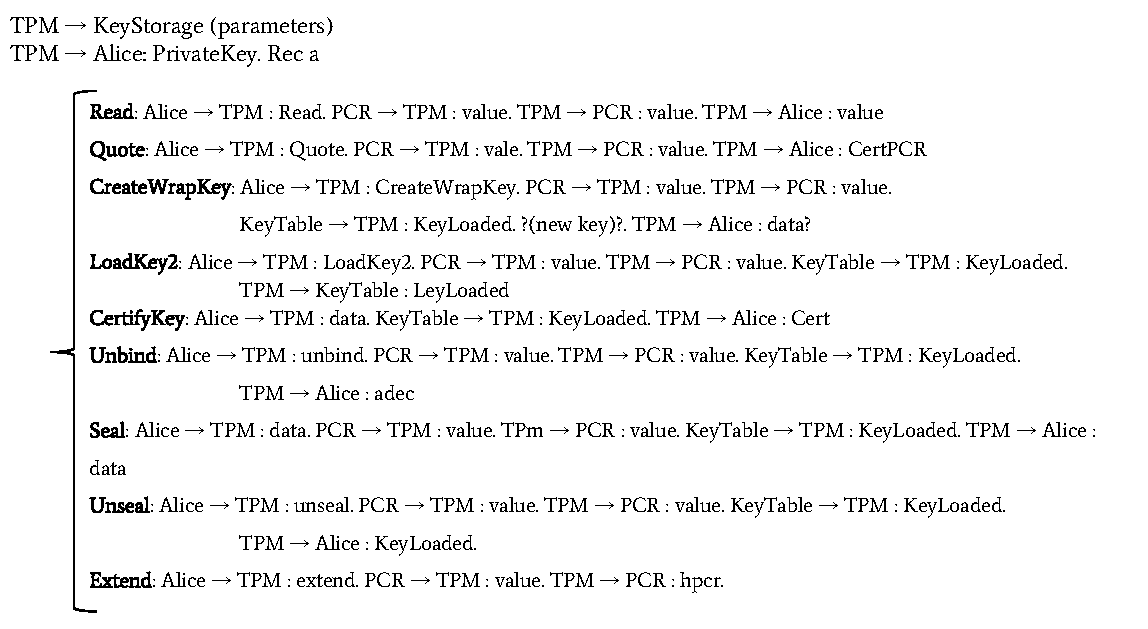
\includegraphics[width=1.2\textwidth, angle=0]{Graphics/Global_Types.pdf}
\end{center}

TODO: Description of above (+ code in appendix? for refs.)